\documentclass[11pt]{article}
\usepackage[margin=2.5cm]{geometry}
\usepackage{tikz}
\usetikzlibrary{arrows.meta, positioning}
\usepackage{array}
\usepackage{tabularx}
\usepackage{booktabs}
\usepackage{enumitem}
\usepackage{hyperref}

% Long identifiers (script/Lambda names) contain underscores but no natural
% break point; without this, a single long \texttt{...} token can overflow
% the page margin instead of wrapping onto the next line.
\renewcommand{\_}{\textunderscore\allowbreak}
\sloppy

\title{Federation Architecture and Implementation\\
\large Digital Twin Microgrid Demo -- Technical Documentation}
\author{}
\date{}

\begin{document}
\maketitle

\section{Overview}

The project implements a federation layer on top of AWS IoT TwinMaker-based
Digital Twins, generated from SysML v2 models via a converter pipeline
(\texttt{digital-twin-profile-sysml-v2} $\rightarrow$ \texttt{digital-twin-manager}).
Federation -- the exchange of data and decisions between independently
deployed twins -- is implemented with \texttt{fed-sysml}, a Terraform-based
generator driven by a single declarative descriptor,
\texttt{pipeline/fed-sysml/input/fedtwin.json}. Each entry in this file
declares one federation Lambda that is triggered by an event on a source
twin, optionally pulls additional data, executes strategy code, and publishes
a result (\emph{feedback}) to a target twin's MQTT ingestion topic.

Two federation groups currently exist in the repository:
\begin{itemize}[nosep]
  \item A pre-existing two-twin push federation between \texttt{dtc2pv} and
        \texttt{dtc2bat} (Section~\ref{sec:legacy}).
  \item A five-twin federation architecture built around
        \texttt{dtcBattery}, \texttt{dtcPV}, \texttt{dtcGrid},
        \texttt{dtcCharger} and \texttt{dtcWeather} (Section~\ref{sec:five-twin}
        onward), which is the current focus of development.
\end{itemize}

\section{Existing Push Federation: dtc2pv $\rightarrow$ dtc2bat}
\label{sec:legacy}

This is the earliest federation in the repository (\texttt{fedTwins} group
\texttt{PVBatteryFederation} in \texttt{fedtwin.json}) and consists of two
independent strategies.

\subsection{dtc-PushUpdateStrategy}
\begin{itemize}[nosep]
  \item \textbf{Source:} \texttt{dtc2pv}, condition \texttt{isGenerating}
        (self-comparison on \texttt{sensor.generatedPower} -- fires on every
        new value).
  \item \textbf{Target:} \texttt{dtc2bat}, component \texttt{pvInput}
        (\texttt{PV\_Virtual\_Sensor}), attribute \texttt{pvGeneratedPower}.
  \item \textbf{Mechanism:} Push. The Collector delivers the triggering
        \texttt{generatedPower} value; the Strategy Lambda
        (\texttt{demo-code/microgrid/fedPvToBatteryPush/lambda\_function.py})
        forwards it unchanged to a hard-coded target device ID (a virtual
        sensor representing PV within the Battery twin), resolved and
        injected by \texttt{scripts/resolve\_federation\_push\_target.py}.
  \item \textbf{Receiving side:} \texttt{dtc2bat} stores the pushed value in
        \texttt{pvInput.pvGeneratedPower}; no condition in \texttt{dtc2bat}
        is defined on this attribute, so it does not itself trigger further
        federation.
\end{itemize}

\subsection{dtc-ConsumptionStrategy}
\begin{itemize}[nosep]
  \item \textbf{Sources:} \texttt{dtc2pv.production} (generatedPower) and
        \texttt{dtc2bat.status} (chargeValue) -- an aggregating strategy
        with two independent triggers.
  \item \textbf{Logic:} \texttt{effective\_consumption = chargeValue - pv\_power}
        (\texttt{demo-code/microgrid/fedTwinCombinedStrategy/lambda\_function.py}).
  \item \textbf{Target:} written back into \texttt{dtc2bat}'s own device
        (\texttt{p16}, attribute \texttt{consumption}) via the federation's
        \texttt{INTERNAL} feedback topic \texttt{dtc2bat/iot-data}.
\end{itemize}

Both strategies publish to the same feedback topic
(\texttt{dtc2bat/iot-data}, \texttt{FEEDBACK\_TYPE = INTERNAL}) and share the
same generated pipeline-Lambda pattern described in Section~\ref{sec:impl}.
This federation is structurally simpler than the five-twin architecture: it
has no Pull step and no cross-twin decision logic -- both strategies are pure
push/aggregate operations.

\section{Five-Twin Federation Architecture}
\label{sec:five-twin}

\subsection{The Five Digital Twins}

The five twins currently modelled in
\texttt{pipeline/digital-twin-profile-sysml-v2/input/} are:

\begin{itemize}[nosep]
  \item \textbf{dtcBattery} -- battery storage: charge level
        (\texttt{charge}), plug state (\texttt{isPlugged}), and externally
        received inputs (\texttt{generatedPower}, \texttt{greenEnergy-}
        \texttt{Percentage}, \texttt{electricityPrice}, \texttt{maxPower}).
  \item \textbf{dtcPV} -- photovoltaic production: simulation hour
        (\texttt{hours\_cycle}) and computed \texttt{production}.
  \item \textbf{dtcGrid} -- grid state: \texttt{greenEnergyPercentage},
        \texttt{currentElectricityPrice}, \texttt{gridLimit},
        \texttt{maxPower}.
  \item \textbf{dtcCharger} -- EV charging point: plug state
        (\texttt{isPlugged}) and the two values it receives from the
        federation, \texttt{actChargeEV} and \texttt{actBatteryCharge}.
  \item \textbf{dtcWeather} -- passive twin holding a fixed hourly solar
        availability lookup table (\texttt{hour00}--\texttt{hour23}, constant
        attributes only); it defines no condition and no strategy action.
\end{itemize}

\subsection{Attribute Reference}
\label{sec:attributes}

The table below consolidates every measure/constant attribute of the five
twins with where its value comes from and what, if anything, currently reads
it. ``Simulator'' denotes a value written by the twin's own simulated
sensor, independent of federation.

\begin{center}
\footnotesize
\setlength{\tabcolsep}{3pt}
\renewcommand{\arraystretch}{1.25}
\begin{tabularx}{\textwidth}{
  @{}>{\raggedright\arraybackslash}p{1.6cm}
  >{\raggedright\arraybackslash}p{2.5cm}
  >{\raggedright\arraybackslash}X
  >{\raggedright\arraybackslash}X@{}
}
\toprule
\textbf{Twin} & \textbf{Attribute} & \textbf{Written by} & \textbf{Read / used by} \\
\midrule
dtcBattery & \texttt{charge} & Simulator (initial); recomputed by the decision federation (\texttt{\_publish\_battery\_state}) & Decision federation (Pull, state-of-charge integration) \\
dtcBattery & \texttt{isPlugged} & ChargerBatteryFederation (push) & Decision federation (trigger + Pull) \\
dtcBattery & \texttt{chargingStatus} & Simulator only & Not consumed by any federation \\
dtcBattery & \texttt{gridPower} & Decision federation (\texttt{\_publish\_battery\_state}) & Not re-consumed by any federation (telemetry only) \\
dtcBattery & \texttt{externalInputs.} \texttt{generatedPower} & PVBatteryGeneratedPowerFederation (push) & Decision federation (trigger + Pull) \\
dtcBattery & \texttt{externalInputs.greenEnergy-} \texttt{Percentage} & GridBatteryFederation (push, \texttt{greenEnergyUpdate}) & Decision federation (trigger + Pull) \\
dtcBattery & \texttt{externalInputs.} \texttt{electricityPrice} & Not written by any current federation & -- (decision federation pulls the price directly from dtcGrid instead; this attribute is currently unused) \\
dtcBattery & \texttt{externalInputs.maxPower} & GridBatteryFederation (push, \texttt{maxPowerUpdate}) & Decision federation (Pull) \\
dtcBattery & \texttt{totalCapacity}, \texttt{maxChargingPower}, \texttt{maxDischargingPower} (consts) & Fixed at deploy (\texttt{initValue}) & Injected as env vars by \texttt{federate\_battery\_charger\_decision.py} \\
\midrule
dtcPV & \texttt{hours\_cycle} & Simulator & PVWeatherFederation (trigger) \\
dtcPV & \texttt{production} & PVWeatherFederation (feedback) & Triggers PVBatteryGeneratedPowerFederation (push onward to Battery) \\
dtcPV & \texttt{maxPower} (const) & Fixed at deploy & Injected as env var by \texttt{federate\_pv\_weather.py} \\
\midrule
dtcGrid & \texttt{greenEnergyPercentage} & Simulator & GridBatteryFederation (push source) \\
dtcGrid & \texttt{currentElectricityPrice} & Simulator & Decision federation (Pull) \\
dtcGrid & \texttt{maxPower} & Simulator & GridBatteryFederation (push source) \\
dtcGrid & \texttt{gridLimit} & Simulator & Not read by any current federation \\
\midrule
dtcCharger & \texttt{isPlugged} & Simulator & ChargerBatteryFederation (push source) \\
dtcCharger & \texttt{actChargeEV} & Decision federation (feedback) & -- (consumed outside federation, e.g.\ simulator/display) \\
dtcCharger & \texttt{actBatteryCharge} & Decision federation (feedback, same message as \texttt{actChargeEV}) & -- (consumed outside federation) \\
dtcCharger & \texttt{maxPower} (const) & Fixed at deploy & Injected as env var by \texttt{federate\_battery\_charger\_decision.py} \\
\midrule
dtcWeather & \texttt{hour00}--\texttt{hour23} (consts) & Fixed at deploy (hardcoded forecast table) & PVWeatherFederation (Pull/Request, one property per invocation) \\
\bottomrule
\end{tabularx}
\end{center}

Two attributes are declared but structurally unused by the current
federation set: \texttt{dtcBattery.externalInputs.electricityPrice} (the
decision federation reads the price directly from \texttt{dtcGrid} via Pull
and never persists it into Battery) and \texttt{dtcGrid.gridLimit} (no
condition or federation references it). This is stated explicitly here
rather than assumed to be wired up.

\subsection{Communication Topology}

Every cross-twin data exchange in this architecture was verified against
\texttt{fedtwin.json} and the corresponding Strategy Lambda source. The twins
do \emph{not} form a fully connected graph: \texttt{dtcCharger} and
\texttt{dtcPV}, \texttt{dtcCharger} and \texttt{dtcGrid},
\texttt{dtcWeather} and any twin other than \texttt{dtcPV} have no direct
federation relationship.

\begin{center}
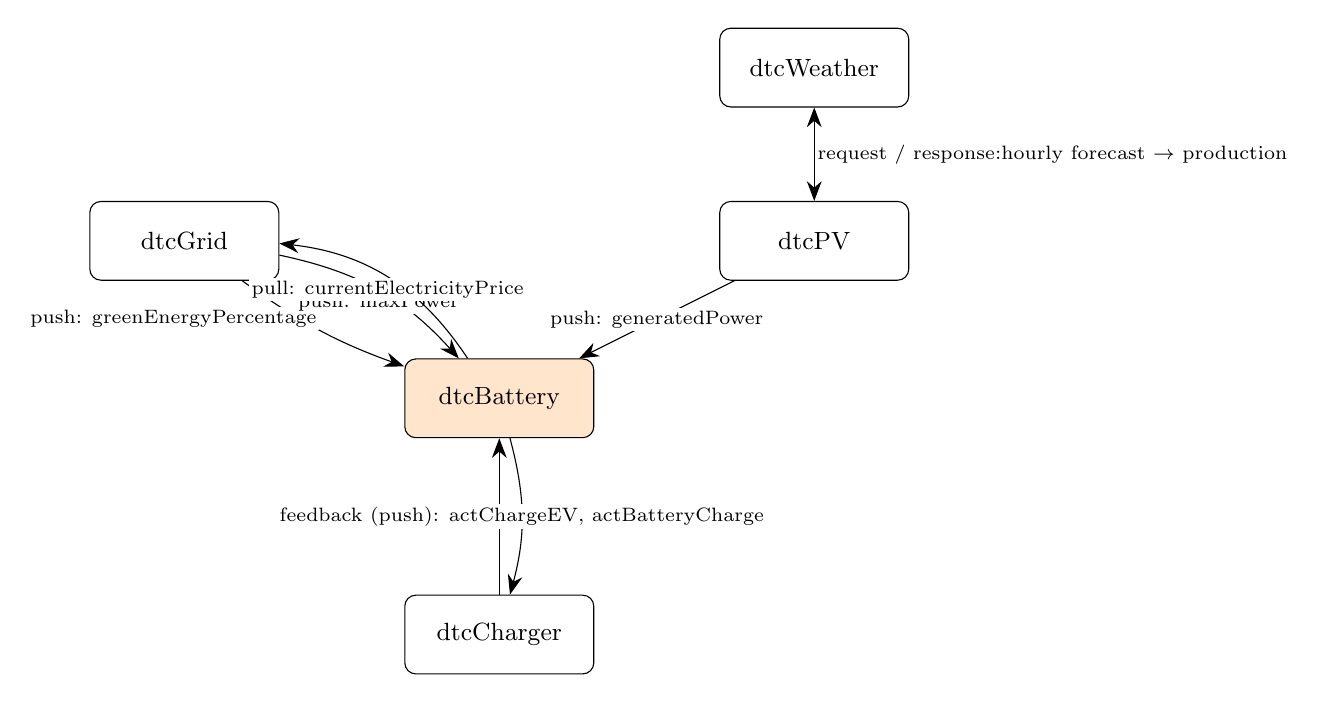
\begin{tikzpicture}[
  twin/.style={draw, rounded corners, minimum width=2.4cm, minimum height=1cm, align=center, font=\small},
  >={Stealth[length=2.5mm]},
  every edge/.style={draw, ->, thick},
  elabel/.style={font=\scriptsize, fill=white, inner sep=1pt}
]
  \node[twin, fill=orange!20] (bat) at (0,0) {dtcBattery};
  \node[twin] (grid) at (-4,2) {dtcGrid};
  \node[twin] (pv)   at (4,2)  {dtcPV};
  \node[twin] (chg)  at (0,-3) {dtcCharger};
  \node[twin] (wea)  at (4,4.2) {dtcWeather};

  \draw[->] (grid) to[bend right=8] node[elabel, above left]{push: greenEnergyPercentage} (bat);
  \draw[->] (grid) to[bend left=18] node[elabel, below]{push: maxPower} (bat);
  \draw[->] (pv) to node[elabel]{push: generatedPower} (bat);
  \draw[->] (chg) to node[elabel]{push: isPlugged} (bat);
  \draw[->] (bat) to[bend left=15] node[elabel]{feedback (push): actChargeEV,\ actBatteryCharge} (chg);
  \draw[->] (bat) to[bend right=25] node[elabel, below]{pull: currentElectricityPrice} (grid);
  \draw[<->] (pv) to node[elabel, right]{request / response:\\ hourly forecast $\rightarrow$ production} (wea);
\end{tikzpicture}
\end{center}

\subsection{Central Role of the Battery Twin}

\texttt{dtcBattery} is the architectural centre of the federation:
\begin{itemize}[nosep]
  \item It is the \emph{only} twin that receives pushed data from three
        independent sources (\texttt{dtcGrid} -- two attributes,
        \texttt{dtcPV}, \texttt{dtcCharger}).
  \item It is the \emph{only} twin that additionally performs an active
        \texttt{Pull} (a Request to \texttt{dtcGrid}'s hot-reader for
        \texttt{currentElectricityPrice}) rather than only reacting to
        pushed events.
  \item It is the \emph{only} twin whose federation strategy runs
        decision logic (\texttt{decision\_logic.py}) that combines all
        collected inputs into a result consumed by another twin
        (\texttt{dtcCharger}).
\end{itemize}
No other twin aggregates more than one external input or produces a
decision consumed elsewhere; this asymmetry is what justifies treating
\texttt{dtcBattery} as the central/decision-making twin rather than an
architectural choice stated explicitly anywhere in the code.

\section{Federation Communication Modes}
\label{sec:modes}

\begin{center}
\footnotesize
\setlength{\tabcolsep}{3pt}
\renewcommand{\arraystretch}{1.3}
\begin{tabularx}{\textwidth}{
  @{}>{\raggedright\arraybackslash}p{1.55cm}
  >{\raggedright\arraybackslash}p{1.55cm}
  >{\raggedright\arraybackslash}p{1.7cm}
  >{\raggedright\arraybackslash}X
  >{\raggedright\arraybackslash}X@{}
}
\toprule
\textbf{Source} & \textbf{Target} & \textbf{Mode} & \textbf{Trigger} & \textbf{Data} \\
\midrule
dtcGrid & dtcBattery & Push & \texttt{greenEnergyUpdate} (self-comp.\ on \texttt{greenEnergyPercentage}) & \texttt{greenEnergyPercentage} \\
dtcGrid & dtcBattery & Push & \texttt{maxPowerUpdate} (self-comp.\ on \texttt{maxPower}) & \texttt{maxPower} \\
dtcPV & dtcBattery & Push & \texttt{productionUpdate} (self-comp.\ on \texttt{production}) & \texttt{generatedPower} \\
dtcCharger & dtcBattery & Push & \texttt{plugUpdate} (self-comp.\ on \texttt{isPlugged}) & \texttt{isPlugged} \\
dtcPV & dtcWeather & Request/ Response & \texttt{isCycling} (self-comp.\ on \texttt{hours\_cycle}) & Request: hour index $\rightarrow$ Response: \texttt{hourNN} forecast \% \\
dtcBattery & dtcGrid & Pull & invoked from within \texttt{plugDecision} strategy execution & \texttt{currentElectricityPrice} \\
dtcBattery & dtcCharger & Push (feedback) & \texttt{plugDecision} / \texttt{surplusDecision} / \texttt{greenEnergyDecision} & \texttt{actChargeEV}, \texttt{actBatteryCharge} \\
\bottomrule
\end{tabularx}
\end{center}

Note that \texttt{dtcBattery}'s decision federation is triggered by any of
three independent conditions (a plug event, a new PV value, or a new grid
green-energy value), all of which point to the same Strategy Lambda -- the
condition only decides \emph{when} the decision re-runs, not what data it
uses; all inputs are re-read fresh on every invocation (see
Section~\ref{sec:impl}).

\subsection{PV $\leftrightarrow$ Weather: Request/Response Detail}

\texttt{dtcPV} triggers on every new \texttt{hours\_cycle} value (0--23).
The federation Strategy Lambda
(\texttt{fedPvWeatherRequest/lambda\_function.py}) converts the hour into a
property name (\texttt{hourNN}) and synchronously invokes
\texttt{dtcWeather}'s hot-reader Lambda for that single constant --
i.e.\ a direct request/response call, not a subscription. The returned
forecast percentage is combined with \texttt{dtcPV}'s own \texttt{maxPower}
constant (\texttt{production = maxPower * forecast / 100}), and the result is
published back to \texttt{dtcPV.panel.production} through the federation's
\texttt{INTERNAL} feedback (\texttt{dtcPV/iot-data}). This is the only
Request/Response relationship in the five-twin architecture; every other
inter-twin exchange is either an unconditional Push or, in Battery's case, a
Pull performed as part of decision execution.

\section{Federation Implementation}
\label{sec:impl}

\subsection{Generated Infrastructure}

\texttt{fed-sysml} reads \texttt{fedtwin.json} and generates
\texttt{pipeline/fed-sysml/output/main.tf}. Per federation strategy this
produces:
\begin{itemize}[nosep]
  \item One \texttt{aws\_lambda\_function} named
        \texttt{<strategyName>\_pipeline} (Python 3.13), which internally
        performs Collector $\rightarrow$ Strategy code $\rightarrow$
        Feedback in a single invocation. There is no separate Step Function
        or separate Collector/Strategy/Feedback Lambda in the currently
        generated infrastructure.
  \item One IAM role/policy granting CloudWatch Logs, scoped
        \texttt{lambda:InvokeFunction} on the hot-reader(s) of the twin(s)
        listed in the strategy's \texttt{strategies} array, and
        \texttt{iot:Publish}.
  \item One \texttt{PARAMETERS} environment variable (JSON) describing what
        the embedded Collector must fetch: property name, data type, the
        originating strategy/action name, and the triggering twin's
        hot-reader ARN/workspace/entity/component.
  \item \texttt{FEEDBACK\_TYPE} (\texttt{INTERNAL} in every current
        federation) and \texttt{FEEDBACK\_TOPIC}
        (\texttt{<targetTwinName>/iot-data}) environment variables, consumed
        by the embedded Feedback step, which calls the AWS IoT Data Plane
        (\texttt{iot-data client}) \texttt{publish(topic, payload)} -- a
        genuine MQTT publish on the target twin's own ingestion topic, not a
        write to a separate analytics store.
  \item One \texttt{aws\_ssm\_parameter} per triggering condition, at
        \texttt{/<twin>/event-registry/<action>}, holding the list of target
        Lambda ARNs to invoke. This SSM parameter tree is the Event
        Registry: it is what an twin's own event-checker consults to know
        which federation Lambda(s) to invoke when one of its conditions
        fires.
\end{itemize}

\subsection{Execution Flow}

\[
\text{Trigger event on source twin}
\;\rightarrow\;
\text{Event Registry lookup (SSM)}
\;\rightarrow\;
\text{Pipeline Lambda: Collector}
\;\rightarrow\;
\text{Strategy code}
\;\rightarrow\;
\text{Feedback (MQTT publish)}
\;\rightarrow\;
\text{Target twin ingestion}
\]

The Collector step fetches the triggering property's current value from the
source twin's hot-reader and hands it to the Strategy code as
\texttt{\{strategyName: \{actionName: \{...\}\}}\}, which every Strategy
Lambda in the repository parses via a small \texttt{\_collector\_payload}
helper. Pure push/passthrough strategies (Grid$\rightarrow$Battery,
PV$\rightarrow$Battery, Charger$\rightarrow$Battery) do nothing beyond
relabelling this payload under the target device ID. Strategies that need
data \emph{not} covered by the Collector (a constant, or a value from a
different twin) read it explicitly via an additional, synchronous
\texttt{lambda\_client.invoke} call to that twin's hot-reader -- this is the
Pull/Request mechanism used by the PV/Weather and Battery/Charger-decision
federations.

\subsection{Federation Enablement Scripts}

\texttt{fed-sysml} can only wire a federation using twin-owned
\texttt{strategyAction}s declared in the \texttt{strategies} array; it cannot
express a hard-coded target device ID, a constant value, or a dependency on
a twin not listed there. These gaps are closed by standalone Python scripts
under \texttt{scripts/}, which fall into two groups with different execution
requirements.

\paragraph{Run manually, once per deployment (\texttt{resolve\_*.py}).}
These edit a target device ID directly into a Strategy Lambda's source
\emph{before} \texttt{continue fed-sysml} packages it, so they must run
\emph{before} \texttt{fed terraform apply}, and are \textbf{not} invoked by
the orchestrator -- they have to be run by hand every time their target
twin is redeployed and its device IDs change:
\begin{itemize}[nosep]
  \item \texttt{resolve\_federation\_push\_target.py} -- \texttt{dtc2bat}'s
        virtual-sensor device ID, into
        \texttt{fedPvToBatteryPush/lambda\_function.py} (legacy federation,
        Section~\ref{sec:legacy}).
  \item \texttt{resolve\_grid\_battery\_push\_target.py} -- \texttt{dtcBattery}'s
        \texttt{greenEnergyPercentage} device ID, into
        \texttt{fedGridToBatteryPush}.
  \item \texttt{resolve\_grid\_battery\_maxpower\_target.py} --
        \texttt{dtcBattery}'s \texttt{maxPower} device ID, into
        \texttt{fedGridToBatteryMaxPowerPush}.
  \item \texttt{resolve\_pv\_battery\_generatedpower\_target.py} --
        \texttt{dtcBattery}'s \texttt{generatedPower} device ID, into
        \texttt{fedPvToBatteryGeneratedPowerPush}.
  \item \texttt{resolve\_charger\_battery\_plug\_target.py} --
        \texttt{dtcBattery}'s \texttt{isPlugged} device ID, into
        \texttt{fedChargerToBatteryPlugPush}.
\end{itemize}

\paragraph{Run automatically by the orchestrator (\texttt{federate\_*.py}).}
\texttt{scripts/orchestrator/pipeline.py} calls
\texttt{federate\_pv\_weather.main()} and
\texttt{federate\_battery\_charger\_decision.main()} itself, \emph{after}
\texttt{fed terraform apply} completes, so these two do not need to be run
by hand as part of the normal pipeline flow:
\begin{itemize}[nosep]
  \item \texttt{federate\_pv\_weather.py} -- injects
        \texttt{dtcWeather}'s hot-reader coordinates and \texttt{dtcPV}'s
        \texttt{maxPower} constant as environment variables on
        \texttt{dtc-PVWeatherStrategy\_pipeline}, and grants it
        \texttt{lambda:InvokeFunction} on \texttt{dtcWeather}'s hot-reader.
  \item \texttt{federate\_battery\_charger\_decision.py} -- injects
        \texttt{dtcGrid}'s and \texttt{dtcBattery}'s hot-reader coordinates,
        the Charger target device ID, and Battery/Charger constant values
        onto \texttt{dtc-BatteryChargerDecisionStrategy\_pipeline}, and
        grants it \texttt{lambda:InvokeFunction} on both hot-readers.
\end{itemize}
They must be re-run (automatically, via the orchestrator, or manually if run
outside it) after \emph{every} Terraform apply that touches their
federation, since \texttt{fed-sysml} only declares
\texttt{PARAMETERS}/\texttt{FEEDBACK\_TYPE}/\texttt{FEEDBACK\_TOPIC} in
\texttt{main.tf} and overwrites the Lambda's environment on each apply --
the injected values do not survive an apply on their own.

\paragraph{Practical implication.} Only the two \texttt{federate\_*.py}
federations self-heal after a Terraform apply. The four push federations
into \texttt{dtcBattery} plus the legacy \texttt{dtc2pv}$\to$\texttt{dtc2bat}
push (five \texttt{resolve\_*.py} scripts in total) require a manual step
every time; skipping it leaves the Strategy Lambda publishing to a stale or
placeholder device ID.

\subsection{Ingestion and Storage}

Independently of federation, each deployed twin has an IoT Topic Rule
(\texttt{SELECT * FROM '<topic>'}) that routes messages on its ingestion
topic to a dispatcher Lambda, which persists values to a hot store queried
later by the twin's hot-reader Lambda (used both by TwinMaker and by the
Pull calls described above). Federation feedback and simulator-originated
messages share the same ingestion topic and are distinguished only by which
attributes are present in the payload / which device ID they target.

\section{Currently Implemented Functionality}

\begin{itemize}[nosep]
  \item Five-twin Digital Twin federation (\texttt{dtcBattery},
        \texttt{dtcPV}, \texttt{dtcGrid}, \texttt{dtcCharger},
        \texttt{dtcWeather}), generated end-to-end from \texttt{fedtwin.json}
        via \texttt{fed-sysml}/Terraform.
  \item Push-based attribute propagation (Grid $\rightarrow$ Battery
        $\times 2$, PV $\rightarrow$ Battery, Charger $\rightarrow$
        Battery).
  \item Pull-based, on-demand read from another twin's hot-reader
        (Battery $\rightarrow$ Grid electricity price).
  \item Request/Response exchange with a dynamic, trigger-dependent query
        (PV $\rightarrow$ Weather hourly forecast).
  \item EV charging decision logic (\texttt{decision\_logic.py}): an energy
        balance that splits available power between the EV and the battery
        with EV priority, branching on whether the grid's green-energy
        share is above a configurable threshold (\texttt{GREEN\_ENERGY\_-}
        \texttt{THRESHOLD = 75.0}), and factoring in electricity price
        (\texttt{price\_factor}) and battery state of charge (reserve /
        full gating).
  \item Battery state-of-charge integration over time
        (\texttt{next\_state\_of\_charge}), with a bounded, accelerated
        simulation clock (\texttt{TIME\_ACCELERATION = 120}).
  \item Renewable-energy-share-driven branching (green-grid vs.\ brown-grid
        charging strategy) and a fixed hourly solar-availability forecast
        table for production forecasting.
  \item Charger/Battery interaction via feedback: the decision federation
        writes both \texttt{actChargeEV} and \texttt{actBatteryCharge} to
        \texttt{dtcCharger} in a single message.
  \item Internal feedback mechanism (\texttt{FEEDBACK\_TYPE = INTERNAL}),
        publishing directly to the target twin's own MQTT ingestion topic
        (\texttt{<twin>/iot-data}) via the AWS IoT Data Plane.
\end{itemize}

No reference to a Siemens use case or a dedicated charging-point-station
twin was found anywhere in the current repository; if this exists, it is not
yet part of the code base covered by this document.

\section{Federation Scenarios}

The following five scenarios correspond directly to the five
\texttt{fedTwins} groups in \texttt{fedtwin.json} that involve the five-twin
architecture (the legacy \texttt{PVBatteryFederation} group, covered in
Section~\ref{sec:legacy}, is excluded here).

\begin{enumerate}[leftmargin=*]
  \item \textbf{GridBatteryFederation.} Twins: \texttt{dtcGrid},
        \texttt{dtcBattery}. Mode: Push (two independent strategies).
        Purpose: keep the Battery twin's view of grid renewable share and
        available grid capacity current. Data: \texttt{greenEnergyPercentage},
        \texttt{maxPower}. Result: both values land in
        \texttt{dtcBattery.externalInputs} and become inputs to the
        charging decision.
  \item \textbf{PVWeatherFederation.} Twins: \texttt{dtcPV},
        \texttt{dtcWeather}. Mode: Request/Response. Purpose: forecast PV
        production for the current simulated hour from a fixed solar
        lookup table. Data: hour index (request) / forecast percentage
        (response). Result: \texttt{dtcPV.production} is (re)computed and
        published, which in turn triggers the next scenario.
  \item \textbf{PVBatteryGeneratedPowerFederation.} Twins: \texttt{dtcPV},
        \texttt{dtcBattery}. Mode: Push. Purpose: forward PV output to the
        Battery twin as an available-power input. Data:
        \texttt{generatedPower} (from \texttt{dtcPV.production}). Result:
        available for the charging decision as PV contribution.
  \item \textbf{ChargerBatteryFederation.} Twins: \texttt{dtcCharger},
        \texttt{dtcBattery}. Mode: Push. Purpose: inform the Battery twin
        that an EV is connected. Data: \texttt{isPlugged}. Result: gates
        whether the decision federation computes a non-zero charging split.
  \item \textbf{BatteryChargingDecisionFederation.} Twins:
        \texttt{dtcBattery}, \texttt{dtcGrid} (Pull), \texttt{dtcCharger}
        (feedback target). Mode: mixed -- triggered by push-delivered
        state, augmented by an explicit Pull, resolved by decision logic,
        delivered by Push/feedback. Purpose: compute the actual EV/battery
        power split. Data in: \texttt{isPlugged}, \texttt{charge},
        \texttt{generatedPower}, \texttt{greenEnergyPercentage},
        \texttt{maxPower} (all pulled with a time range from Battery's own
        hot storage), \texttt{currentElectricityPrice} (pulled from Grid).
        Data out: \texttt{actChargeEV}, \texttt{actBatteryCharge} to
        \texttt{dtcCharger}, plus a separate direct publish of the updated
        \texttt{charge} and \texttt{gridPower} back into
        \texttt{dtcBattery}'s own topic.
\end{enumerate}

\section{Twin Responsibilities}

\begin{itemize}[nosep]
  \item \textbf{dtcBattery} -- aggregates every external input in the
        architecture, owns the only cross-twin decision logic, tracks and
        integrates its own state of charge, and is the sole source of the
        Charger's control values. Functions as the federation's decision
        engine.
  \item \textbf{dtcPV} -- produces a derived attribute
        (\texttt{production}) from an external source (Weather) and
        forwards it onward (Battery); does not consume any pushed data
        itself.
  \item \textbf{dtcGrid} -- pure source twin: exposes renewable share,
        capacity and price; only ever pushed from or pulled from, never a
        receiver of federation output.
  \item \textbf{dtcCharger} -- pure sink for the decision output
        (\texttt{actChargeEV}, \texttt{actBatteryCharge}); its own plug
        state is the only value it contributes, pushed onward to Battery.
  \item \textbf{dtcWeather} -- passive data source with no condition or
        strategy action of its own; participates only as the target of
        PV's Request/Response calls.
\end{itemize}

\section{Federation Architecture Summary}

The current federation layer connects five Digital Twins --
\texttt{dtcBattery}, \texttt{dtcPV}, \texttt{dtcGrid}, \texttt{dtcCharger}
and \texttt{dtcWeather} -- using three distinct interaction patterns: Push
(Grid$\rightarrow$Battery, PV$\rightarrow$Battery,
Charger$\rightarrow$Battery, and Battery$\rightarrow$Charger feedback),
Pull (Battery$\rightarrow$Grid, on demand, as part of decision execution),
and Request/Response (PV$\leftrightarrow$Weather, a synchronous,
trigger-parameterised query). The twin graph is intentionally sparse:
\texttt{dtcCharger} and \texttt{dtcGrid} never exchange data directly with
\texttt{dtcPV} or with each other, and \texttt{dtcWeather} is reachable only
from \texttt{dtcPV}. \texttt{dtcBattery} is structurally central -- it is the
only node with in-degree greater than one, the only twin that issues a
Pull rather than only reacting to pushes, and the only twin whose federation
Lambda executes decision logic that fuses multiple sources
(renewable share, price, PV production, plug state, own state of charge)
into a single control output consumed by another twin. Each federation is
generated as one self-contained AWS Lambda (Collector, Strategy and Feedback
executed in-process) from a declarative \texttt{fedtwin.json} entry, with an
SSM-parameter-based Event Registry dispatching triggering events to the
correct Lambda(s), and INTERNAL feedback delivered as a direct MQTT publish
to the target twin's own ingestion topic. This combination -- a sparse,
asymmetric topology with one aggregating/decision-making twin and three
distinct, explicitly-typed exchange modes -- is what the five-twin
architecture demonstrates as a federation pattern beyond the earlier,
purely push-based dtc2pv/dtc2bat implementation.

\end{document}
